\documentclass[tikz,border=5mm]{standalone}
\usepackage{tikz}
\usepackage{etoolbox}
\usetikzlibrary{positioning,matrix,backgrounds,calc}


\pgfdeclarelayer{background}
\pgfdeclarelayer{foreground}
\pgfsetlayers{background,main,foreground}

\definecolor{sindynullgray}{RGB}{200,200,200}
\definecolor{sindyforces}{RGB}{196,78,82}
\definecolor{sindynewton}{RGB}{85,168,104}
\definecolor{sindylagrange}{RGB}{129,114,179}

\newcommand{\lb}{[}
\newcommand{\rb}{]}

% Define the sindy component as a node style
\tikzset{
    sindy label/.style={font=\tiny, text=black,minimum height=0pt},
    sindy component/.style={
        rectangle,
        minimum width=10pt,
        minimum height=1.5cm,
        rounded corners=5pt,
        fill=none,
        draw=none,
        inner sep=0pt,
        outer sep=1pt,
        align=center,
    },
    with label/.style={label={[sindy label]above:#1}}
}

\begin{document}
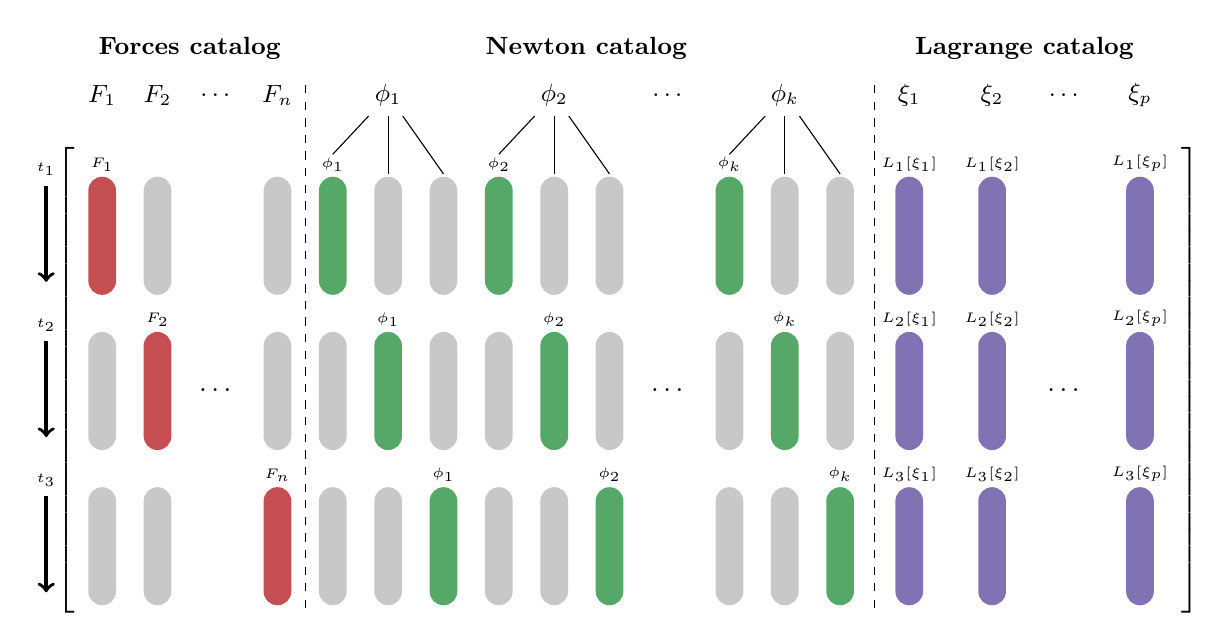
\begin{tikzpicture}

%Create a matrix of nodes with automatic naming (m-row-column)
\matrix[matrix of nodes,
        column sep=10pt, 
        row sep=0.2cm,
        nodes={sindy component},
        left delimiter={[},
        right delimiter={]},
        nodes in empty cells
        ] (m) {
    |[fill=sindyforces,with label=$F_1$]| & |[fill=sindynullgray]| &  & |[fill=sindynullgray]| & |[fill=sindynewton,with label=$\phi_1$]| & |[fill=sindynullgray]| & |[fill=sindynullgray]| & |[fill=sindynewton,with label=$\phi_2$]| & |[fill=sindynullgray]| & |[fill=sindynullgray]| & & |[fill=sindynewton,with label=$\phi_k$]| & |[fill=sindynullgray]| & |[fill=sindynullgray]| & |[fill=sindylagrange,with label=$L_1 \lb \xi_1 \rb$]| & |[fill=sindylagrange,with label=$L_1 \lb \xi_2 \rb$]| & & |[fill=sindylagrange,with label=$L_1 \lb \xi_p \rb$]| \\
    |[fill=sindynullgray]| & |[fill=sindyforces,with label=$F_2$]| & |[fill=none]|\dots  & |[fill=sindynullgray]| & |[fill=sindynullgray]| & |[fill=sindynewton,with label=$\phi_1$]| & |[fill=sindynullgray]| & |[fill=sindynullgray]| & |[fill=sindynewton,with label=$\phi_2$]| & |[fill=sindynullgray]| & |[fill=none]|\dots & |[fill=sindynullgray]| & |[fill=sindynewton,with label=$\phi_k$]| & |[fill=sindynullgray]| & |[fill=sindylagrange,with label=$L_2 \lb \xi_1 \rb$]| & |[fill=sindylagrange,with label=$L_2 \lb \xi_2 \rb$]| & |[fill=none]|\dots & |[fill=sindylagrange,with label=$L_2 \lb \xi_p \rb$]| \\
    |[fill=sindynullgray]| & |[fill=sindynullgray]| &   & |[fill=sindyforces,with label=$F_n$]| & |[fill=sindynullgray]| & |[fill=sindynullgray]| & |[fill=sindynewton,with label=$\phi_1$]| & |[fill=sindynullgray]| & |[fill=sindynullgray]| & |[fill=sindynewton,with label=$\phi_2$]| &  & |[fill=sindynullgray]| & |[fill=sindynullgray]| & |[fill=sindynewton,with label=$\phi_k$]| & |[fill=sindylagrange,with label=$L_3 \lb \xi_1 \rb$]| & |[fill=sindylagrange,with label=$L_3 \lb \xi_2 \rb$]| &  & |[fill=sindylagrange,with label=$L_3 \lb \xi_p \rb$]| \\
    };

\draw[dashed] ($(m-3-4.south east)!0.5!(m-3-5.south west)$) -- ($(m-1-4.north east)!0.5!(m-1-5.north west)$) -- ++(0,1.2cm);

\draw[dashed] ($(m-3-14.south east)!0.5!(m-3-15.south west)$) -- ($(m-1-14.north east)!0.5!(m-1-15.north west)$) -- ++(0,1.2cm);

\node at ($(m-1-1.north)!0.5!(m-1-4.north) + (0,1.6cm)$) {\small \textbf{Forces catalog}};
\node at ($(m-1-5.north)!0.5!(m-1-14.north) + (0,1.6cm)$) {\small \textbf{Newton catalog}};
\node at ($(m-1-15.north)!0.5!(m-1-18.north) + (0,1.6cm)$) {\small \textbf{Lagrange catalog}};

\node at ($(m-1-1.north) + (0,1cm)$) {\small $F_1$};
\node at ($(m-1-2.north) + (0,1cm)$) {\small $F_2$};
\node at ($(m-1-3.north) + (0,1cm)$) {\small \dots};
\node at ($(m-1-4.north) + (0,1cm)$) {\small $F_n$};

\node (phi1-label) at ($(m-1-6.north) + (0,1cm)$) {\small $\phi_1$};
\node (phi2-label)at ($(m-1-9.north) + (0,1cm)$) {\small $\phi_2$};
\node at ($(m-1-11.north) + (0,1cm)$) {\small \dots};
\node (phi3-label)at ($(m-1-13.north) + (0,1cm)$) {\small $\phi_k$};

\draw (phi1-label) -- ($(m-1-5.north) + (0,0.25cm)$);
\draw (phi1-label) -- (m-1-6.north);
\draw (phi1-label) -- (m-1-7.north);

\draw (phi2-label) -- ($(m-1-8.north) + (0,0.25cm)$);
\draw (phi2-label) -- (m-1-9.north);
\draw (phi2-label) -- (m-1-10.north);

\draw (phi3-label) -- ($(m-1-12.north) + (0,0.25cm)$);
\draw (phi3-label) -- (m-1-13.north);
\draw (phi3-label) -- (m-1-14.north);

\node at ($(m-1-15.north) + (0,1cm)$) {\small $\xi_1$};
\node at ($(m-1-16.north) + (0,1cm)$) {\small $\xi_2$};
\node at ($(m-1-17.north) + (0,1cm)$) {\small \dots};
\node at ($(m-1-18.north) + (0,1cm)$) {\small $\xi_p$};

\node[anchor=south] at ($(m-1-1.north west) + (-0.5cm,-0.15cm)$) {\tiny $t_1$};
\draw[->,line width=1.25pt] ($(m-1-1.north west) + (-0.5cm,-0.15cm)$) -- ($(m-1-1.south west) + (-0.5cm,0.2cm)$);

\node[anchor=south] at ($(m-2-1.north west) + (-0.5cm,-0.15cm)$) {\tiny $t_2$};
\draw[->,line width=1.25pt] ($(m-2-1.north west) + (-0.5cm,-0.15cm)$) -- ($(m-2-1.south west) + (-0.5cm,0.2cm)$);

\node[anchor=south] at ($(m-3-1.north west) + (-0.5cm,-0.15cm)$) {\tiny $t_3$};
\draw[->,line width=1.25pt] ($(m-3-1.north west) + (-0.5cm,-0.15cm)$) -- ($(m-3-1.south west) + (-0.5cm,0.2cm)$);

\end{tikzpicture}
\end{document}